\documentclass[times, utf8, diplomski]{fer}
\usepackage{booktabs}
\usepackage[final]{pdfpages}

\begin{document}

% TODO: Navedite broj rada.
\thesisnumber{2345}

\title{Proceduralno generiranje trave i niskog raslinja}
\author{Mihael Međan}

\maketitle

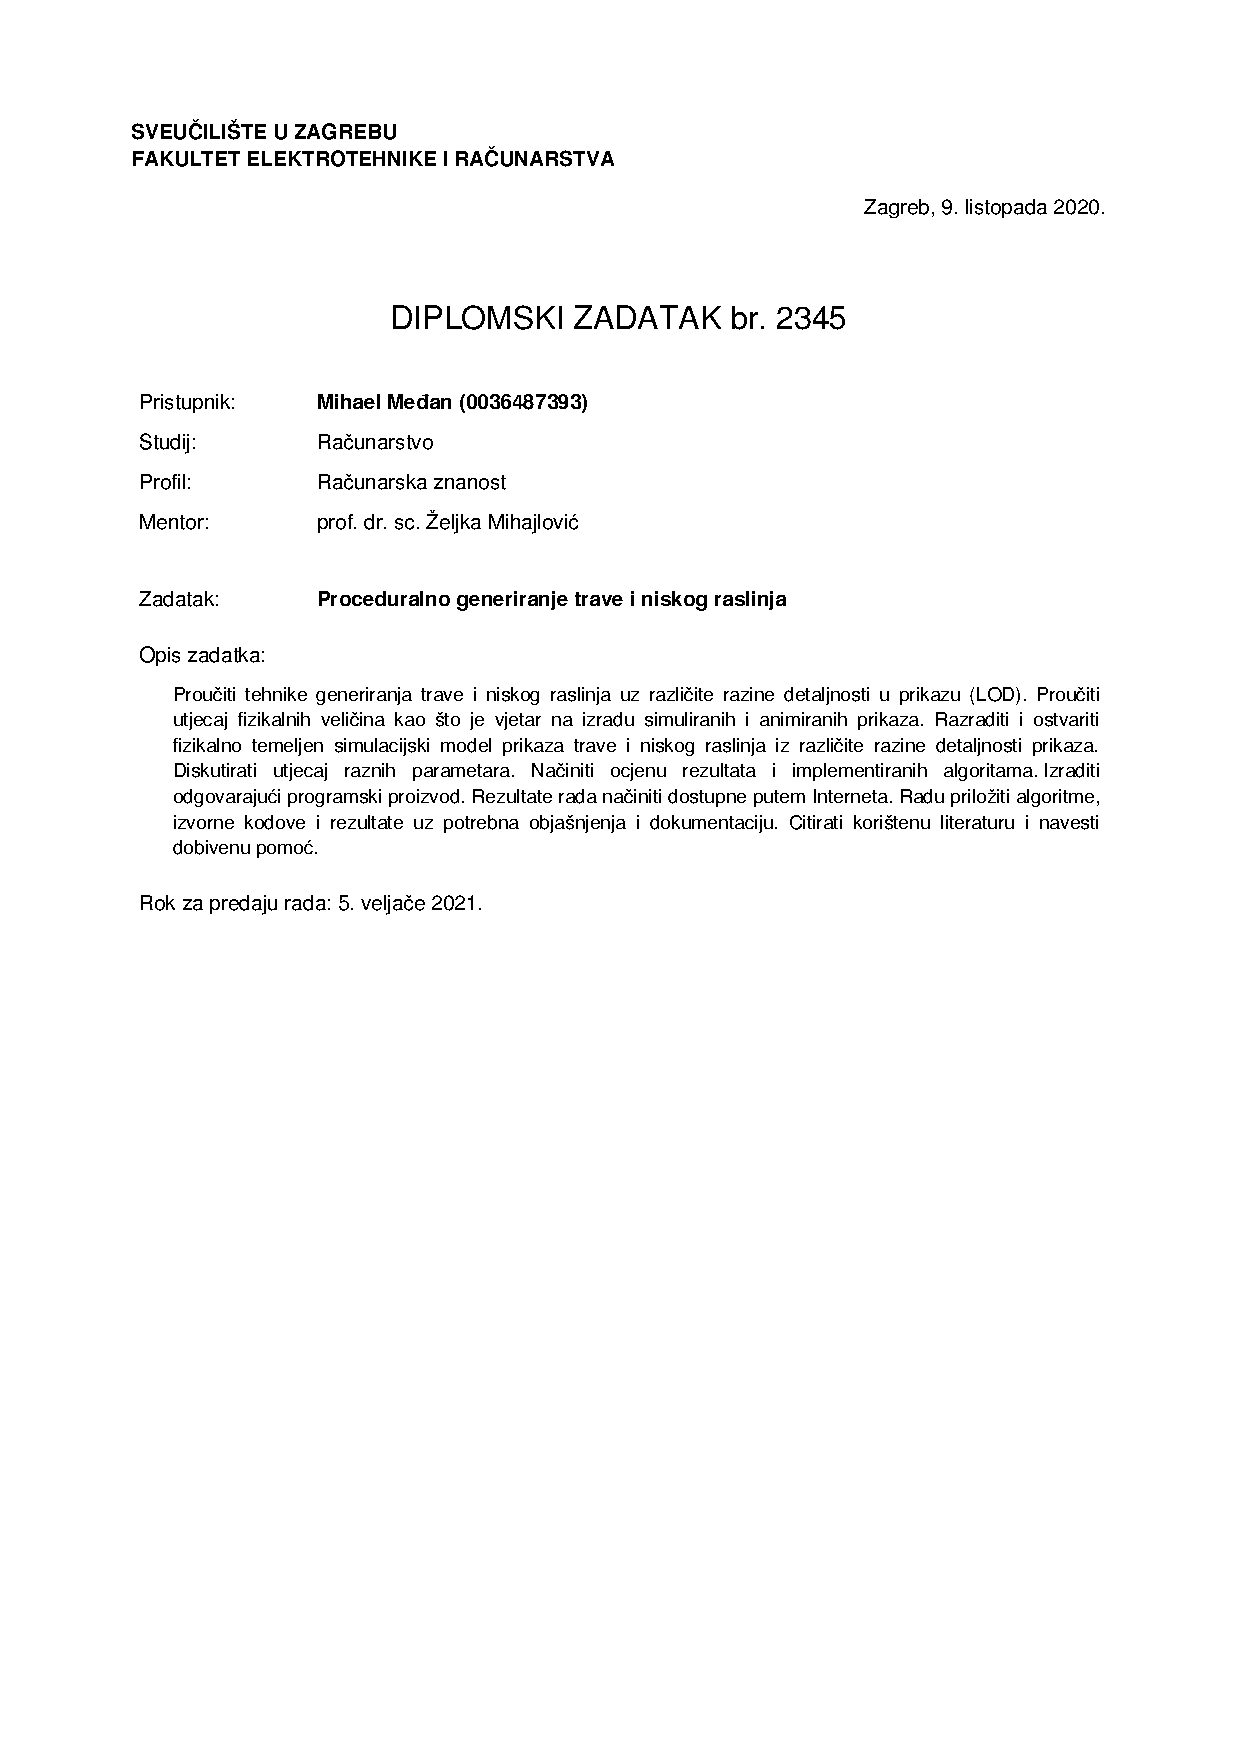
\includepdf[pages=-,offset=0 -75]{hr_0036487393_56.pdf}

\zahvala{}

\tableofcontents

\chapter{Uvod}
Uvod rada. Nakon uvoda dolaze poglavlja u kojima se obrađuje tema.

\chapter{Generiranje modela trave i niskog raslinja}
\section{Osnovni pristup generiranju modela}

\section{Generiranje točaka i poligona modela biljaka}

\subsection{Generiranje modela uz različitu razinu detalja}

\section{Povezivanje generiranih podataka i njihov prikaz}

\section{Programska implementacija generiranja i prikaza}

\section{Primjer korištenja razvijenog programa za generiranje jednostavne proizvoljne biljke}

\chapter{Simulacijski model}
\section{Fizički model ponašanja biljke}
\paragraph{}
Osnovne sile koje utječu na ponašanje biljke su sila teža, unutrašnji otpor 
biljke i vanjski utjecaji. Sila teža konstantnim intenzitetom gura sve dijelove 
biljke prema dolje. Vanjski utjecaji poput vjetra, djeluju u svim smjerovima 
različitim intenzitetima na različite dijelove biljke. Te unutrašnji otpor 
biljke, koji uvijek dijeluje u suprotnom smjeru od preostale dvije sile. Na 
slici \ref{fig:31-1} su slikovito prikazane kumulativne sile koje u nekom 
trenutku djeluju na biljku.

\begin{figure}[h]
	\centering
	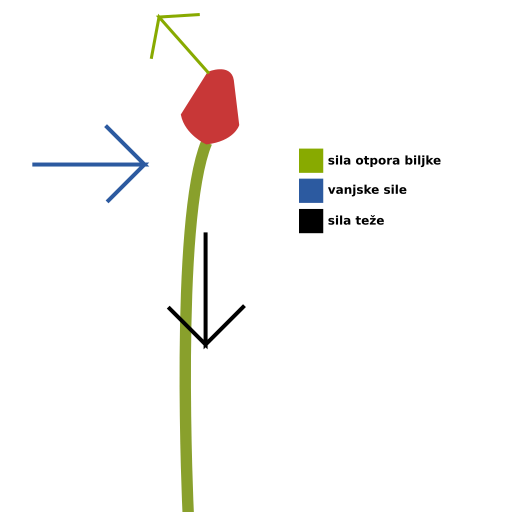
\includegraphics[width=0.8\textwidth]{img/31-1}
	\caption{Prikaz sila koje djeluju na biljku}
	\label{fig:31-1}
\end{figure}

\paragraph{}
Usred djelovanja te tri sile, biljka u svakom trenutku pokušava doći u stanje gdje se te tri sile poništavaju. Svako gibanje biljke prouzrokovano je promjenom vanjskih utjecaja kojima se biljka pokuša prilagoditi kako bi ukupna sila koja djeluje na biljku bila nula.

\paragraph{}
Čak i naizgled jednostavan problem kao što je simuliranje ponašanja biljke je u svojoj 
naravi izrazito kompleksan. Sila teža djeluje na svaki mikroskopsi dio biljke. Na isti način
djeluju i vanjske sile. Vanjske sile i sila teže u biljci uzrokuju napetosti i kompresije 
koje uzrokuju silu otpora biljke. To sve se događa na mikroskopskoj razini na svakom dijelu 
površine biljke. Savršena simlacija ovakvog sustava bila bi izrazito računalno zahtjevna.

\section{Programski model fizičkog ponašanja}
\paragraph{}
Zbog računalne zahtjevnosti i problema preciznog definiranja svih sila, potrebno je pronaći
matematički model koji bi rezultirao istim (ili barem vrlo sličnim) ponašanjem, a imao bi 
mnogo manju računalnu složenost i bio bi jednostavniji za definirati.

\paragraph{}
U računalnom programiranju se fizičke interakcije obično modeliraju preko tri osnovna  
građevna bloka. Tijela, ograničenja i sile. Tijela su geometrijski oblici u tro-
dimenzijskom prostoru koja zauzimaju volumen i podložna su dijelovanju sila. Ograničenja 
su skup pravila koja određuju kako se neka dva tijela mogu ponašati relativno jedno prema 
drugom. Sile dijeluju na tijela i uzrokuju promjene koje se tada na temelju ograničenja 
rješavaju.

\paragraph{}
Primjer tijela je kocka u trodimenzijskom prostoru. Primjer sile je sila teža koja djeluje 
konstantnim intenzitetom prema negativnoj y osi. Primjer ograničenja je ako se volumen 
jednog tijela nađe unutar volumena drugog tijela, na oba tijela se primjenjuje sila u smjeru 
suprotnom od središta mase drugog tijela. Ovo ograničenje je naivni pristup riješavanju 
kolizija između tijela.

\paragraph{}
Stvarnu simulaciju jednostavne biljke možemo vrlo dobro aproksimirati korištenjem svega dva tijela, jednog ograničenja i jedne sile koja dijeluje na jedno od tijela.

\section{Programska implementacija fizičkog modela}

\section{Implementacije fizičkog ponašanja složenih biljaka}

\chapter{Simulacija ponašanja generiranog modela}
\section{Povezivanje fizičkog modela sa generiranim prikazom modela}

\section{Programska implementacija modela}

\section{Utjecaj parametara na simulaciju}

\chapter{Ocjena rezultata}
\section{Realističnost prikaza}
\paragraph{}
Realističnost prikaza nije bila primarna zadaća ovog rada. Generirane biljke ne 
izgledaju osobito prirodno bez obzira na razinu detalja kojom su generirane. Primjer generiranih biljaka vidljiv je na slici \ref{fig:51-1}.
\begin{figure}[h]
	\centering
	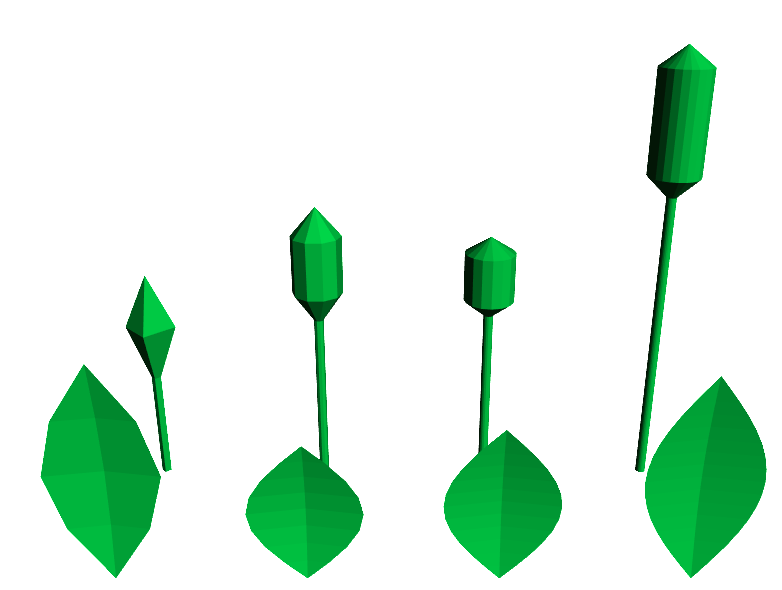
\includegraphics[width=0.8\textwidth]{img/51-1}
	\caption{Prikaz modela u različitoj razini detalja}
	\label{fig:51-1}
\end{figure}
\paragraph{}
Prvi razlog je primjena konstantnog sjenčanja poligona. U ovakvom načinu 
sjenčanja, normale za pojedine vrhove računamo kao normalu površine (poligona)
kojeg oni zatvaraju. Izračunata vrijednost normale se pripisuje svim vrhovima
poligona. Korištenjem konstantnog sjenčanja poligona postižemo jasno 
vidljivu granicu između pojedinih površina. Takav način prikaza, osim što je
vrlo brz u izvođenju, znatno je olakšao razvoj prezentiranog programskog 
rješenja jer daje programeru jasan uvid u poziciju pojedinih vrhova na ekranu
i njihovo ponašanje. 

\paragraph{}
Bez obzira na prednosti u razvoju koje ovakav pristup implicira, prikazani 
modeli izgledaju umjetno i izrazito su pravilni. Pravilnost modela je najveći
uzrok neprirodnog izgleda generiranih modela, jer na biljkama rijetko očekujemo
savršenu simetriju oko geometrijskih osi.
\paragraph{}
Drugi razlog je nedostatak detalja na generiranim modelima biljaka. Ovaj razlog 
dodatno naglašava pravilnost biljaka i smanjuje osjećaj realnosti prikaza.
Smanjenje broja detalja donijelo je iste prednosti kao i prethodni pristup - 
lakši razvoj i bolje performanse po cijenu realističnosti prikaza.
\paragraph{}
Treći razlog je izolacija prikaza. Biljke su prikazane kao centralni i jedini 
dio prikaza. Ovakav vakuum u prostoru dodatno naglašava oba prije spomenuta 
problema. Nedostatak simulacije atmosfere (prašina, distorzija zraka svjetlosti 
kao posljedica vlage u zraku itd.) uzrokuje dojam statičnosti biljaka bez
obzira na animirani prikaz ponašanja vjetra. Izostavak navedenih značajki, kao
i prethodna pojednostavljenja, olakšalo je razvoj programskog rješenja i 
oslobodilo vrijeme za ostvarenje kvalitetnije simulacije vjetra.

\subsection{Mogućnosti poboljšanja}
\paragraph{}
Problem sjenčanja može se riješiti primjenom nekog drugog načina sjenčanja 
modela. Naprimjer korištenje Gouraudovog sjenčanja. Korištenje ove metode 
sjenčanja eliminiralo bi vidljivost pojedinih vrhova na modelu i interpolacijom
između vrhova osiguralo gladak prijelaz između osjenčanih i ne osjenčanih 
dijelova modela. 
\paragraph{}
Biljke u stvarnosti rijetko imaju ikakve oštre bridove između svojih strana i 
zaglađivanje intenziteta osvjetljenja Gouraudovog sjenčanja između vrhova bi 
rezultiralo uvjerljivijim prikazom kod modela generiranih u većoj razini 
detalja. Kod modela generiranih manjom razinom detalja, rubovi samog modela bi
ostali oštri iako je model zaglađen. Sraz između rubova i unutrašnjosti modela
može uzrokovati smanjenje realističnosti prikaza.
\paragraph{}
Dodavanje malih varijacija kod generiranja modela poboljšalo bi realističnost 
prikaza. Mali istupi točaka od centra simetrije dali bi biljkama prirodniji
izgled uvođenjem nesavršenosti i raznovrsnosti biljaka. Osim dodavanja istupa
u poziciji točaka u modelu, istupi se mogu dodati i na boje pojedinih površina,
gdje bi neke površine bile više ili manje intenzivne boje od drugih. Dodavanje
boja u kombinaciji s Gouraudovim sjenčanjem dodatno bi pojačalo realističnost
prikaza.
\paragraph{}
Dodavanje varijacija je programski izrazito jednostavno za implementaciju ali
uzrokuje usporenje izvođenja, jer se svaki model zbog svoje unikatnosti mora
preslikati u memoriju grafičke kartice umjesto korištenja istog modela za sve 
biljke iste vrste. Kompromis se može postići na sredini - imati limitiran broj 
različitih modela iste vrste biljke koji se nasumično odabere za svaku biljku 
prilikom njenog kreiranja.
\paragraph{}
Dodavanje atmosferskih efekata na simulaciju bi uvelike pomoglo realističnosti
prikaza i dojmu živosti biljaka. Ovaj pristup riješavanju nerealističnosti 
prikaza je najkompleksniji od ponuđenih alternativa i zahtjeva razvoj nekolicine 
popratnih sustava, ali dao bi najveći doprinos realističnosti prikaza. Primjeri 
popratnih sustava koje je potrebno razviti uključuju: sustav ukrasnih čestica, 
sustav efekata nakon iscrtavanja (engl. \textit{post-processing effects}) i 
druge. 

\section{Realističnost fizičke simulacije}
\paragraph{}
Bez obzira na jednostavnost implementacije fizičke simulacije i snažne
pretpostavke uključene u nju, fizička simulacija daje zadovoljavajuće rezultate.
Ponašanje prati stvarno prirodno gibanje u tri dimenzije i ne potiče osjećaj 
umjetnosti ili ograničenosti prolaskom kroz prostor. Simulacija dobro modelira
utjecaj visine biljke na njezinu simulaciju na vjetru. 
\paragraph{}
Na udarima vjetra visoke biljke rade velike i snažne zamahe i polagano gube 
energiju za nastavak daljnjeg osciliranja. Niske biljke rade kraće zamahe ali 
većom frekvencijom.
\paragraph{}
Kod konstantnog puhanja, biljke osciliraju prema točki konvergencije sile 
puhanja, sile teže i sila otpora unutar stabljke. Visoke biljke očekivano imaju veću amplitudu i manju frekvenciju oko te točke od niskih biljaka.
\paragraph{}
Puhanje s naletima vjetra također daje realistične rezultate. Niske biljke u 
naletu vjetra se brzo poravnavaju prema točki konvergencije i osciliraju oko 
nje, a po prestanku puhanja osciliraju oko centra ravnoteže velikom 
frekvencijom. Visoke biljke imaju veću tromost i rade veće oscilacije oko točke
konvergencije vjetra i otpora biljke prilikom naleta vjetra. Kad vjetar 
prestane, naprave manje oscilacija oko centra ravnoteže prije nego vjetar 
ponovno počne.
\begin{figure}[h]
	\centering
	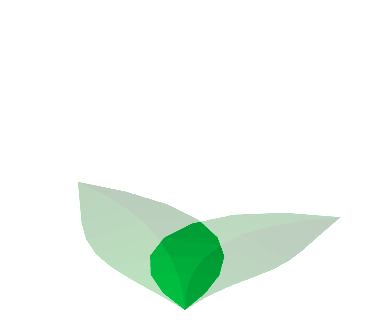
\includegraphics[width=0.4\textwidth]{img/52-1}
	\caption{Katično ponasanje niske biljke prilikom vjetra u valovima}
	\label{fig:52-1}
\end{figure}
\paragraph{}
Kad je simulacija vjetra realistična (takva da vjetar dolazi i prolazi u 
valovima - postepeno raste u snazi, i nakon toga postepeno opada u snazi) 
također imamo realističnu simulaciju. Visoke biljke održavaju smjer i neprestano 
osciliraju prema središtu između točaka centra ravnoteže otpora biljke, i 
konvergentne točke sile vjetra, ravnoteže i unutarnjeg otpora biljke. Niske 
biljke kod ovakvog vjetra djeluju kaotično i osciliraju velikom frekvencijom i 
amplitudom, sa središtem oscilacije koji vidno varira između konvergentne točke 
i centra ravnoteže biljke. Razlika u ponašanju je vidljiva na slikama \ref{fig:52-1} i \ref{fig:52-2}
\begin{figure}[h]
	\centering
	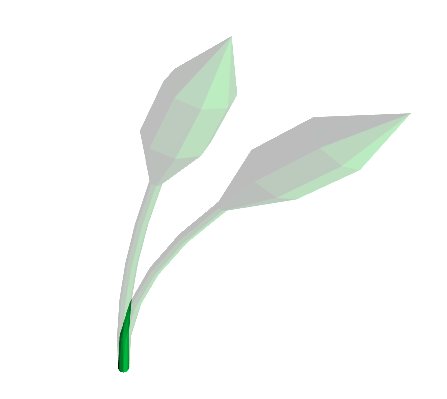
\includegraphics[width=0.4\textwidth]{img/52-2}
	\caption{Stabilno ponasanje visoke biljke prilikom vjetra u valovima}
	\label{fig:52-2}
\end{figure}

\subsection{Poboljšanje realističnosti simulacije}
\paragraph{}
Još realističnija simulacija se može postići dodavanjem većeg broja zglobova u
fizički kostur biljke. Dodavanjem većeg broja zglobova dobili bi mogućnost 
simulacije pregiba u stabljci biljke. U prirodi kod jednostavnih biljaka ovaj 
fenomen nije uvijek jasno vidljiv, ali možemo ga uočiti kad je vjetar u 
rezonantnoj frekvenciji sa stabljkom biljke.
\paragraph{}
Dodatnu kontrolu možemo postići dodavanjem težina pojedinim zglobovima. Tako da 
na neke dijelove kostura vjetar ima jači utjecaj nego na druge. Primjer takve 
biljke je zvončić, kod kojeg je utjecaj vjetra puno jasnije vidljiv na cvijetu 
nego na stabljci biljke.

\section{Brzina izvođenja}
\paragraph{}
Brzina izvođenja linearno opada s brojem simuliranih biljaka. Najveći utjecaj na 
brzinu izvođenja ima fizička simulacija. Generiranje biljaka se odvija na samom 
početku i nema nikakvog utjecaja na brzinu izvođenja nakon početnog perioda 
generiranja. Iscrtavanje je zbog jednostavnosti prikaza vrlo jeftino i usporava
izvođenje tek na velikom broju biljaka ili na vrlo visokoj razini detalja. Graf trajanja vremenkog koraka vidljiv je na \ref{fig:53-1}.
\begin{figure}[h]
	\centering
	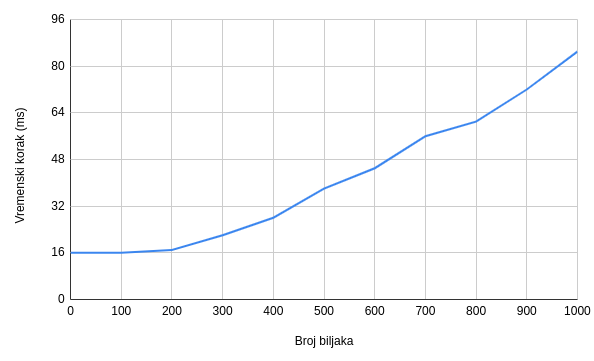
\includegraphics[width=0.95\textwidth]{img/53-1}
	\caption{Trajanje vremenskog koraka u ovisnosti o broju biljaka u simulaciji}
	\label{fig:53-1}
\end{figure}

\subsection{Pristupi poboljšanju brzine izvođenja}
\paragraph{}
Fizička simulacija ima najveći utjecaj na brzinu izvođenja pa su prijedlozi za 
ubrzanje programskog rješenja fokusirani na taj dio.
\subsubsection{Paralelno izvođenje fizičke simulacije}
\paragraph{}
Trenutna programska implementacija u obzir uzima i kolizije samih biljaka. 
Fizička simulacija se odvija slijedno za svaku od biljaka i eventualni dodir 
nakon simulacije neke od narednih biljaka moće imati utjecaj na onu prvu. Ako
ne marimo za interakciju između samih biljaka i odlučimo je zanemariti, 
jednostavan način za ubrzanje fizičke simulacije je paralelizam. Na \ref{fig:531-1} je prikazan dijagram slijednog i paralelnog izvođenja (na dvije dretve) i vidljivo je da paralelni primjer završava u dva koraka dok slijedni algoritam završava u jednom koraku.

\begin{figure}[h]
	\centering
	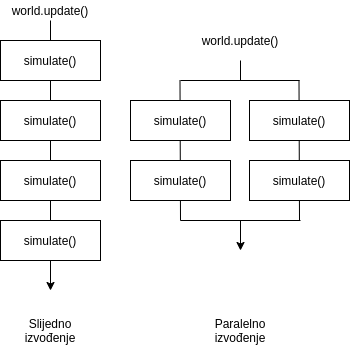
\includegraphics[width=0.7\textwidth]{img/531-1}
	\caption{Dijagram slijednog i paralelnog izvođenja}
	\label{fig:531-1}
\end{figure}
\paragraph{}
Na ovaj način svaka biljka (ili grupa biljaka) može imati svoj fizički procesor 
koji će se brinuti o njezinoj simulaciji i cijeli proces se završava u manje 
koraka.

\subsubsection{Smanjenje rezolucije simulacije i zaglađivanje rezultata}
\paragraph{}
Brzinu izvođenja možemo i povećati na način da ne ažuriramo fizičku simulaciju 
biljke u svakom koraku. Kod ovakvog pristupa stanje svake biljke izračunavamo 
nakon nekoliko koraka umjesto na svakom, a rezultate u međukoracima zagladimo.
U primjeru \ref{fig:531-2} vidimo slijed simulacije jedne biljke kroz vremenske 
korake. Prilikom simulacije trebamo osigurati da je vremenski razmak za koji 
simuliramo točno onoliko koraka koliko će trajati do sljedeće simulacije i to 
uzrokuje smanjenje reyolucije simulacije. Ako bi vremenski korak simulacije 
ostao jednak kao da simuliramo biljku u svakom simulacija bi se odvijala 
usporeno.
\paragraph{}
Bitno je ostvariti da se nikad istovremeno ne simuliraju i zaglađuju svi modeli 
nego da je postupak naizmjeničan. Za primjer sa dvije biljke, dok se jedna 
biljka simulira druga se zaglađuje i obratno.
\begin{figure}[h]
	\centering
	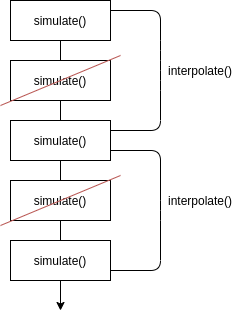
\includegraphics[width=0.5\textwidth]{img/531-2}
	\caption{Dijagram simulacije sa zaglađivanjem}
	\label{fig:531-2}
\end{figure}
\paragraph{}
Problem kod ovakvog pristupa je kašnjenje prikaza nad stvarnim stanjem fizičke 
simulacije. Fizička simulacija je uvijek barem jedan korak ispred prikaza. Ovo 
može uzrokovati naizgledno podrhtavanje ukoliko želimo zadržati simulaciju 
interakcija između biljaka, a biljka se pomaknula nakon što je dobivena zadnja 
točka za interpolaciju. Ako ne marimo za interakciju između biljaka, ovaj 
problem možemo zanemariti. Iako će animacija i dalje kasniti za stvarnim 
fizičkim stanjem, promatraču to neće biti vidljivo.
\subsubsection{Izračunavanje sličnosti modela i grupiranje izračuna}
\paragraph{}
Ukoliko nam nije bitna interakcija između biljaka i želimo drastično smanjiti utjecaj fizičke simulacije na brzinu izvođenja možemo izdvojiti prototipne biljke iz simulacije i simulirati samo njih. Sve ostale biljke, ovisno o sličnosti će koristiti podatke simulacije te biljke kao svoje. Primjer takvog sustava vidljiv je na slici \ref{fig:531-3}
\begin{figure}[h]
	\centering
	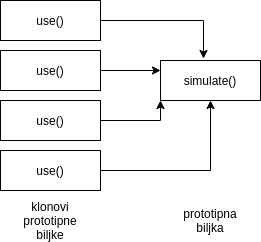
\includegraphics[width=0.5\textwidth]{img/531-3}
	\caption{Dijagram simulacije sa zaglađivanjem}
	\label{fig:531-3}
\end{figure}
\paragraph{}
Na ovaj način potrebno je simulirati samo nekoliko biljaka umjesto svih ali ovakav pristup će rezultirati time da simulacija izgleda nerealistično jer će sličnosti između ponašanja biljaka biti identične u isto vrijeme i na istim uvjetima što narušava dojam realizma. Potencijalno rješenje ovog problema je da kod nekih biljaka unesemo kašnjenje nad prototipnom biljkom. Na taj način smo eliminirali problem dojma da se sve ponavlja, ali smo uveli problem da simulacija ne djeluje toliko responzivno.

\chapter{Zaključak}
ma moze se sve buraz kad se oce

\listoffigures

\bibliography{literatura}
\bibliographystyle{fer}

\begin{sazetak}
Sažetak na hrvatskom jeziku.

\kljucnerijeci{Ključne riječi, odvojene zarezima.}
\end{sazetak}

% TODO: Navedite naslov na engleskom jeziku.
\engtitle{Procedural generation of grass and low vegetation}
\begin{abstract}
Abstract.

\keywords{Keywords.}
\end{abstract}

\end{document}
